%===============================================================================
% LaTeX sjabloon voor de bachelorproef toegepaste informatica aan HOGENT
% Meer info op https://github.com/HoGentTIN/bachproef-latex-sjabloon
%===============================================================================

\documentclass{bachproef-tin}

\usepackage{hogent-thesis-titlepage} % Titelpagina conform aan HOGENT huisstijl
\usepackage{epigraph}
\setlength\epigraphrule{0pt}
% Packages van de student
\usepackage{subcaption}
\usepackage{pdfpages}
\usepackage[overload]{textcase}
\usepackage[acronym]{glossaries}

\makeglossaries

\newacronym{acr:ux}{UX}{User Experience}
\newacronym{acr:ui}{UI}{User Interface}
\newacronym{acr:uxd}{UXD}{User Experience Design}
\newacronym{acr:gui}{GUI}{Grafische User Interface}
\newacronym{acr:cli}{CLI}{Command Line Interface}
\newacronym{acr:sus}{SUS}{System Usability Scale}
\newacronym{acr:roi}{ROI}{Return on Investment}
\newacronym{acr:cta}{CTA}{Call-To-Action}
\newacronym{acr:faq}{FAQ}{Frequently Asked Questions}

%%---------- Documenteigenschappen ---------------------------------------------
% TODO: Vul dit aan met je eigen info:

% De titel van het rapport/bachelorproef
\title{Een gebruiker wegwijs maken doorheen een applicatie van aanzienlijke omvang}

% Je eigen naam
\author{Jakob Lierman}

% De naam van je promotor (lector van de opleiding)
\promotor{Karine Samyn}

% De naam van je co-promotor. Als je promotor ook je opdrachtgever is en je
% dus ook inhoudelijk begeleidt (en enkel dan!), mag je dit leeg laten.
\copromotor{Bert Maurau}

% Indien je bachelorproef in opdracht van/in samenwerking met een bedrijf of
% externe organisatie geschreven is, geef je hier de naam. Zoniet laat je dit
% zoals het is.
\instelling{Cardify}

% Academiejaar
\academiejaar{2019-2020}

% Examenperiode
%  - 1e semester = 1e examenperiode => 1
%  - 2e semester = 2e examenperiode => 2
%  - tweede zit  = 3e examenperiode => 3
\examenperiode{2}

%===============================================================================
% Inhoud document
%===============================================================================

\begin{document}

%---------- Taalselectie -------------------------------------------------------
% Als je je bachelorproef in het Engels schrijft, haal dan onderstaande regel
% uit commentaar. Let op: de tekst op de voorkaft blijft in het Nederlands, en
% dat is ook de bedoeling!

%\selectlanguage{english}

%---------- Titelblad ----------------------------------------------------------
\inserttitlepage

%---------- Samenvatting, voorwoord --------------------------------------------
\usechapterimagefalse
%%=============================================================================
%% Voorwoord
%%=============================================================================

\chapter*{\IfLanguageName{dutch}{Woord vooraf}{Preface}}
\label{ch:voorwoord}

Deze bachelorproef werd geschreven in het kader van het behalen van het diploma ``Bachelor in de Toegepaste Informatica'', afstudeerrichting Mobile Apps.

Mijn interesses gaan verder dan enkel de technische kant van mijn opleiding. Net daarom heb ik voor dit onderwerp gekozen. Het verkennen van verschillende \acrshort{acr:ux} en \acrshort{acr:ui}-elementen sprak me enorm aan. Het was een leerrijke ervaring om applicaties en IT voor te leggen aan iedereen in mijn omgeving, jong en oud, om dan van dichtbij te observeren hoe men met de technologie omspringt.

Deze scriptie zou niet tot stand zijn gekomen zonder enkele personen. Hierbij wil ik van dit voorwoord graag gebruik maken om deze personen te bedanken. 

Zonder Bert Maurau, mijn co-promotor, had ik deze scriptie niet kunnen aanvullen met gegevens en voorbeelden vanuit Cardify. Hij en Seppe Vereecken stonden steeds klaar om mijn vragen te beantwoorden en deze scriptie aan te vullen met nuttige info en voorbeelden.

Deze scriptie werd geschreven tijdens de Covid-19-crisis. Bram Van de velde heeft tools aangeboden om mijn proef zo vlot mogelijk te laten verlopen vanop afstand. Zo kon ik de proof-of-concept applicatie delen met iPhone-gebruikers zonder hiervoor met de participant in contact te komen.

Quentin Braet gaf deze scriptie een extra dimensie door zijn kennis van bij In The Pocket te delen. Door deze inzichten op te nemen in de tekst is deze scriptie een volwaardig schrijven waar naartoe kan verwezen worden bij de implementatie van of onderzoek naar learnability in software.

Karine Samyn, mijn promotor, volgde mijn voortgang nauw op en gaf op regelmatige basis feedback. Door deze opbouwende kritiek werd deze scriptie zonder veel problemen tot een goed einde gebracht.

Amber Priem hielp me doorheen de statistische analyses, waardoor ik mijn gemeten waardes kon omzetten in een conclusie. Ook was ze steeds de eerste die klaar stond om een tekstblok na te lezen of te controleren op grammaticale fouten.

Ten slotte had ik graag nog mijn ouders bedankt voor de financiële steun om deze opleiding tot een goed einde te brengen. Uiteraard had ik hen en iedereen die mijn scriptie even doornam graag nogmaals bedankt om deze tekst na te lezen, ook al ligt deze uit hun interessegebied.

Ik wens u veel leesplezier toe.

Jakob Lierman

Gent, \shortdate\today



%%=============================================================================
%% Samenvatting
%%=============================================================================

% TODO: De "abstract" of samenvatting is een kernachtige (~ 1 blz. voor een thesis) synthese van het document.

% Deze aspecten moeten zeker aan bod komen:
% - Context: waarom is dit werk belangrijk?
% - Nood: waarom moest dit onderzocht worden?
% - Taak: wat heb je precies gedaan?
% - Object: wat staat in dit document geschreven?
% - Resultaat: wat was het resultaat?
% - Conclusie: wat is/zijn de belangrijkste conclusie(s)?
% - Perspectief: blijven er nog vragen open die in de toekomst nog kunnen onderzocht worden? Wat is een mogelijk vervolg voor jouw onderzoek?

\chapter*{\IfLanguageName{dutch}{Samenvatting}{Abstract}}

Elke gebruiker moet leren werken met de applicaties die hij of zij op zijn of haar toestel installeert. Men kan deze gebruiker helpen door middel van implementatie van learnability-elementen doorheen de software.

De grote meerderheid aan bedrijven en ontwikkelaars hebben echter de tijd of middelen niet om deze technieken zo geoptimaliseerd mogelijk uit te werken. Deze scriptie geeft duidelijkheid over de verschillende mogelijkheden en de effecten ervan. Dit schrijven werd aangevuld met inzichten van ontwikkelaars.

Om het effect van learnability-elementen te meten werd er een usability test uitgevoerd met enkele participanten. Uit dit onderzoek resulteert dat het gebruik van deze elementen wel degelijk voordelig is, als en slechts als deze op de juiste manier verwerkt zijn doorheen de software. Elke software verschilt en voor elke software moet opnieuw bekeken worden waar men best hulp kan voorzien. Dit gaat vlot aan de hand van usability tests doorheen fases van de ontwikkeling.

De relatie tussen (het gebrek aan) in-app user training en de gebruiksduur en/of levensduur van de applicatie wordt aanbevolen als toekomstig onderzoek. Hierbij kan men deze proef als startpunt gebruiken met een gerichte applicatie en een steekproef waarbij elke participant interesse toont in de functionaliteiten van de applicatie.


%---------- Inhoudstafel -------------------------------------------------------
\pagestyle{empty} % Geen hoofding
\tableofcontents  % Voeg de inhoudstafel toe
\cleardoublepage  % Zorg dat volgende hoofstuk op een oneven pagina begint
\pagestyle{fancy} % Zet hoofding opnieuw aan

%---------- Lijst figuren, afkortingen, ... ------------------------------------

% Indien gewenst kan je hier een lijst van figuren/tabellen opgeven. Geef in
% dat geval je figuren/tabellen altijd een korte beschrijving:
%
%  \caption[korte beschrijving]{uitgebreide beschrijving}
%
% De korte beschrijving wordt gebruikt voor deze lijst, de uitgebreide staat bij
% de figuur of tabel zelf.

\listoffigures
\listoftables
\printacronyms

% Als je een lijst van afkortingen of termen wil toevoegen, dan hoort die
% hier thuis. Gebruik bijvoorbeeld de ``glossaries'' package.
% https://www.overleaf.com/learn/latex/Glossaries

%---------- Kern ---------------------------------------------------------------

% De eerste hoofdstukken van een bachelorproef zijn meestal een inleiding op
% het onderwerp, literatuurstudie en verantwoording methodologie.
% Aarzel niet om een meer beschrijvende titel aan deze hoofstukken te geven of
% om bijvoorbeeld de inleiding en/of stand van zaken over meerdere hoofdstukken
% te verspreiden!

%%=============================================================================
%% Inleiding
%%=============================================================================

\chapter{\IfLanguageName{dutch}{Inleiding}{Introduction}}
\label{ch:inleiding}

\epigraph{If the user can't use it, it doesn't work.}{\textit{Susan Dray}}

In digitale tijden als deze is de vraag naar nieuwe software groot. Programmeurs en IT-bedrijven hebben hun handen vol. Zowat elke sector wil mee zijn met de digitale boot. Je komt hedendaags overal software tegen; de computer op het werk, de smartphone in je broekzak, het bedieningspaneel van een grote kraan, de kassa in de supermarkt, $\dots$ Je gebruikt hoogstwaarschijnlijk tal van software in het dagelijkse leven. Maar hoe leer je nu het best omgaan met deze computerprogramma's? Programma's bevatten vaak heel veel functies. Veel van deze functies blijven echter onbenut omdat de gebruiker niet voldoende begrijpt hoe deze functies in zijn werking treden. De programmeurs achter deze software hebben vaak hun handen al vol met het ineen knutselen van al deze functionaliteit waardoor zij zelf geen tijd hebben om te kijken hoe de eindgebruiker met deze functionaliteit omspringt.

\epigraph{How do I explain what I do at a party? The short version is that I say I humanize technology.}{\textit{Fred Beecher, Director of UX, The Nerdery}}

Hier komt de~\acrshort{acr:ux}-designer aan bod. Een~\acrshort{acr:ux}-designer zorgt er voor dat software bruikbaar is voor de eindgebruiker. Taken die zijn job omschrijven omvatten, maar zijn niet beperkt tot, het maken van prototypes, testen van (deel)producten bij gebruikers, observeren van gedrag van gebruikers op bepaalde functionaliteiten en stukken software, \textit{user flows} creëren en ook onderzoek doen naar de doelgebruiker~\autocite{White2020}. De UX-designer zal dus ook een flow creëren dat ervoor zorgt dat de gebruiker alle functionaliteit van de applicatie goed begrijpt en snel onder de knie heeft.

Eén van de bekendste implementaties hiervan is de ``onboarding''. Je komt vaak in contact met onboarding wanneer je de applicatie voor de eerste maal opstart. Zo'n onboarding kan zeer verschillend zijn van applicatie tot applicatie.
Er bestaan uiteraard meer manieren om de gebruiker de weg te wijzen doorheen software. Een simpele \textit{tooltip} of zelfs een help-pagina of leerplatform doet ook wonderen.

\section{\IfLanguageName{dutch}{Probleemstelling}{Problem Statement}}
\label{sec:probleemstelling}

Bij veel software-ontwikkelaars en -designers stelt de vraag zich frequent of een bepaalde implementatie van onboarding of in-app user training wel het gewenste effect bekomt. Er bestaan verscheidene manieren om dit in een applicatie te verwerken, om echter te weten of de ene manier een beter resultaat boekt dan de andere is een onderzoek nodig.

We bekeken de voordelen van onboarding en in-app user training tot nu toe voornamelijk vanuit het oogpunt van de eindgebruiker. Echter kan dit ook effect hebben op andere aspecten binnen een bedrijf. Deze scriptie zal ook de effecten op het klantbehoud analyseren. Er zal dus onderzocht worden of de klant zich meer geneigd gaat voelen een bepaalde applicatie met een andere en/of betere implementatie van de verschillende technieken frequenter te gebruiken.

\section{\IfLanguageName{dutch}{Onderzoeksvraag}{Research question}}
\label{sec:onderzoeksvraag}

\subsection{Hoofdonderzoeksvraag}
\label{sec:hoofdonderzoeksvraag}

Zoals reeds aangehaald in sectie~\ref{sec:probleemstelling} zal dit onderzoek zich focussen op implementaties van onboarding en in-app user training en de gevolgen van deze implementaties. Daaruit vloeit volgende hoofdonderzoeksvraag voort:

\begin{itemize}
    \item Kan een (betere) onboarding en in-app user training ervoor zorgen dat de eindgebruiker een beter inzicht heeft op de totale functionaliteit van een grote applicatie?
\end{itemize}

\subsection{Deelonderzoeksvragen}
\label{sec:deelonderzoeksvragen}

Ter ondersteuning van de hoofdonderzoeksvraag zijn er ook nog enkele deelonderzoeksvragen opgesteld:

\begin{itemize}
    \item Hoe een grote hoeveelheid aan functionaliteiten beheersbaar houden voor de eindgebruiker?
    \item Heeft (het gebrek aan) in-app user training effect op de gebruiksduur en/of levensduur van de applicatie?
    \item Hoe de eindgebruiker wegwijs maken in een grote applicatie?
\end{itemize}

Doorheen deze scriptie zal op deze deelonderzoeksvragen een antwoord geformuleerd worden.

\section{\IfLanguageName{dutch}{Onderzoeksdoelstelling}{Research objective}}
\label{sec:onderzoeksdoelstelling}

Het hoofddoel van dit onderzoek is het aantonen van de werking en gevolgen van verschillende technieken om de eindgebruiker familiair te maken met de applicatie. Door middel van een proof-of-concept zal worden aangetoond welke technieken het meest gewenste resultaat hebben op de eindgebruiker.

Een tweede doel bestaat uit het onderzoeken of (het gebrek aan) deze technieken ook effect heeft op het klantbehoud bij de applicatie.

Een laatste doel is om er voor te zorgen dat ontwikkelaars die dit lezen een idee krijgen van de UX-technieken die men kan gebruiken bij de implementatie van hun applicatie. Daarnaast kunnen UX-designers ook deze scriptie raadplegen bij het uitdenken van hun user flows.

\section{\IfLanguageName{dutch}{Opzet van deze bachelorproef}{Structure of this bachelor thesis}}
\label{sec:opzet-bachelorproef}

De rest van deze bachelorproef is als volgt opgebouwd:

In Hoofdstuk~\ref{ch:stand-van-zaken} wordt een overzicht gegeven van de stand van zaken binnen het onderzoeksdomein, op basis van een literatuurstudie.

In Hoofdstuk~\ref{ch:methodologie} wordt de methodologie toegelicht en worden de gebruikte onderzoekstechnieken besproken om een antwoord te kunnen formuleren op de onderzoeksvragen.

% TODO: Vul hier aan voor je eigen hoofdstukken, één of twee zinnen per hoofdstuk

In Hoofdstuk~\ref{ch:metingen} worden de gemeten waarden uit de proef (visueel) weergegeven.

In Hoofdstuk~\ref{ch:resultaten} formuleert men, met behulp van statistische analyses, de bevindingen die af te leiden zijn uit de metingen.

In Hoofdstuk~\ref{ch:conclusie}, tenslotte, wordt de conclusie gegeven en een antwoord geformuleerd op de onderzoeksvragen. Daarbij wordt ook een aanzet gegeven voor toekomstig onderzoek binnen dit domein.
\chapter{\IfLanguageName{dutch}{Stand van zaken}{State of the art}}
\label{ch:stand-van-zaken}

% Tip: Begin elk hoofdstuk met een paragraaf inleiding die beschrijft hoe dit hoofdstuk past binnen het geheel van de bachelorproef. Geef in het bijzonder aan wat de link is met het vorige en volgende hoofdstuk.

Zoals uit vorig hoofdstuk kan worden afgeleid zal deze scriptie onderzoek doen naar de implementatie en effecten van bepaalde UX en UI-elementen. Maar alvorens van start te gaan hiermee zal eerst gekeken worden naar wat de algemene rol is van UX en UI in software-ontwikkeling.

\section{User experience in software}
\label{sec:user-experience-in-software}

In het traditioneel proces van het ontwikkelen van software staat de functionaliteit centraal. Ontwikkelaars bekijken alle vereisten en starten met de belangrijkste. Functionaliteit krijgt hier doorgaans de voorkeur. \textcite{Harutyunyan2019} stelden vast dat dit de laatste jaren echter aan het wijzigen is. De traditionele softwareontwikkeling is plaats aan het maken voor softwareontwikkeling met user experience in het achterhoofd. Dit fenomeen noemt men User Experience Design of kortweg UXD. Omdat de term UXD in de literatuur nog sterk evolueert heeft dit nog geen algemeen aanvaarde definitie. Men kan stellen dat user experience design een proces is waarbij men gebruiksgedrag zal manipuleren aan de hand van de bruikbaarheid en wenselijkheid in de interactie met een product. 

Men doet al lang onderzoek naar user experience in software. Zo toonden \textcite{Carroll1984} het belang van training in complexe systemen al aan anno 1984. Deze training van gebruikers behandelen we later in dit hoofdstuk.

\begin{figure}[h]
    \centering
    \def\svgwidth{.8\columnwidth}
    \input{./img/user-experience-waarom-wat-hoe.pdf_tex}
    \caption{Het waarom, wat en hoe van user experience design}
    \label{fig:ux-waarom-wat-hoe}
\end{figure}

Een UX-designer bekijkt het product niet enkel als een het product zelf. Deze persoon analyseert hoe de eindgebruiker het product in gebruik neemt en past het product aan zodat de gebruikservaring optimaal is. De designer neemt het \textit{waarom}, \textit{wat} en \textit{hoe} van productgebruik in acht (zie figuur~\ref{fig:ux-waarom-wat-hoe}) \autocite{Hassenzahl2013}. De \textit{wat} in productgebruik verwijst gewoonlijk naar wat een gebruiker kan doen door middel van het product. Dit is bijvoorbeeld ``een foto maken'' of ``een spel kopen''. De \textit{hoe} staat dan ook effectief voor de gebruiker het product gebruikt. Dit is meer op een operationeel niveau zoals het navigeren door software met behulp van knoppen en andere attributen. De designer zal zich voornamelijk focussen op het ``hoe'' van het productgebruik. Dit omvat de gegeven functionaliteit op een aantrekkelijke manier zeer toegankelijk maken.

\section{Belangrijke factoren bij user experience}
\label{sec:belangrijke-factoren-bij-user-experience}

Er zijn talloze factoren die ervoor zorgen dat men op een verschillende manier naar dezelfde applicatie moet kijken. Zo zijn de gebruikers allemaal verschillend, maar er moet ook rekening gehouden worden met verschillende omgevingen, culturen, enz. Een toestel om parameters op te meten bij schepen moet dus waterbestendig zijn. Een kindvriendelijke tablet is best schokbestendig. Een applicatie om notities te maken bij vergaderingen is best geluidsloos.

De factoren kunnen gegroepeerd worden in vijf groepen (zie figuur~\ref{fig:ux-factoren}). Culturele factoren omvatten bijvoorbeeld religie, taal en gewoontes. Zo moet bij het ontwerpen van een website gericht op asielzoekers bijvoorbeeld rekening houden met het gebrek aan kennis van de landstaal.

Een mobiele applicatie waarbij de gebruiker een vervoersbewijs moet voorleggen op een voertuig van het openbaar vervoer zal bijvoorbeeld rekening moeten houden met het feit dat de sociale factor tijdsdruk hier belangrijk is. Indien deze applicatie niet tijdig het vervoersbewijs laat zien zal er een hele wachtrij ontstaan die dan vertragingen tot gevolg heeft.

Je kan factoren met betrekking tot de context waarin het product gebruikt wordt opvatten als bijvoorbeeld tijd en locatie. Bij het bestellen van een pakket krijg je vaak een tracking-link waarbij ook het tijdstip van levering staat. Een internationale leverancier moet dus zeker voorzien dat de tijd van de levering in de juiste tijdzone weergegeven wordt.

De gebruiker zelf verschilt uiteraard ook. Een applicatie gericht op een ouder publiek voorziet best grote tekst en duidelijke iconen.

Het product zelf moet uiteindelijk ook nog bruikbaar zijn en alle functionaliteiten moeten eenvoudig bereikbaar zijn.
Een hele boterham voor de user experience designer om onderzoek naar te doen voor zijn use case.

\begin{figure}
    \centering
    \def\svgwidth{.8\columnwidth}
    \input{./img/user-experience-factoren.pdf_tex}
    \caption{Belangrijke factoren bij user experience}
    \label{fig:ux-factoren}
\end{figure}

\textcite{Morville2004} verdeelde user experience op een andere manier. Hij maakt gebruik van de user experience honingraat (zie figuur~\ref{fig:ux-facets}) die user experience opsplitst in zeven onderdelen.

% TODO - https://www.interaction-design.org/literature/article/the-7-factors-that-influence-user-experience

\begin{itemize}
    \item \textbf{Nuttig.}
    Alle producten moeten een zeker nut hebben. Een applicatie mag niet zomaar een tool zijn van het management maar moet een zekere waarde hebben voor de eindgebruiker.
    \item \textbf{Bruikbaar.}
    De bruikbaarheid of usability van een product is een van de belangrijkste kenmerken van de user experience. Het is echter niet het enige kenmerk. Bruikbaarheid en gebruiksgemak zijn dus essentieel maar niet voldoende.
    \item \textbf{Gewenst.}
    De zoektocht naar een efficiënte applicatie mag de branding, het image en de esthetiek van de applicatie niet achterwege laten. Hoe wenselijker het product is, hoe meer de gebruiker erover zal opscheppen tegen potentieel nieuwe gebruikers.
    \item \textbf{Vindbaar.}
    Software moet eenvoudig te navigeren zijn. Gebruikers moeten vlot kunnen vinden wat ze nodig hebben.
    \item \textbf{Toegankelijk.}
    Software moet toegankelijk zijn voor alle doelgroepen. Een gebruiker met een handicap mag geen hindernissen ondervinden bij het gebruik ervan.
    \item \textbf{Geloofwaardig.}
    De design elementen gebruikt in de software moeten ervoor zorgen dat de gebruikers vertrouwen hebben in de informatie die we hen meedelen.
    \item \textbf{Waardevol.}
    De software moet waarde leveren voor de organisatie. De organisatie zal er naar streven dat de winst en klanttevredenheid sterk toenemen.
\end{itemize}

\begin{figure}
    \centering
    \def\svgwidth{.8\columnwidth}
    \input{./img/user-experience-facets.pdf_tex}
    \caption{De user experience honingraat}
    \label{fig:ux-facets}
\end{figure}

User experience design is een zeer creatief concept. Door deze creativiteit zijn er uiteraard verschillende meningen over hoe men user experience moet definiëren, omschrijven en indelen. Mits de belangrijkste vermeld zijn gaan we hier niet verder op in.

\subsection{User experience design in de praktijk}
\label{sec:user-experience-in-software:user-experience-design-in-de-praktijk}

% https://medium.com/@jtnakagawa/nothing-left-to-take-away-437eb23c2ae8
Een eenvoudige applicatie moet simpel in gebruik zijn, dat is waar \textbf{Medium} (\href{https://medium.com/@jtnakagawa/nothing-left-to-take-away-437eb23c2ae8}{https://medium.com/}) op inzet. Medium is een online platform voor schrijvers en lezers. Bij een blog-artikel moet men focussen op de inhoud van het artikel. Door een gebrek aan kleurgebruik en een goede keuze van het lettertype is Medium gebruiksvriendelijker dan de papieren krant. Afbeeldingen zijn groot en duidelijk, de titel springt eruit en op enkele iconen na zijn er weinig tot geen afleidingen te bespeuren (zie figuur~\ref{fig:ux-voorbeeld-medium:desktop}). Medium trekt deze lijn door naar hun mobiele applicatie (zie figuur~\ref{fig:ux-voorbeeld-medium:mobiel}). Hier implementeerde men ook een donkere variant. Deze variant zorgt voor leescomfort in donkere omgevingen en in sommige gevallen ook voor batterijbesparing \autocite{Jin2017}.

\begin{figure}
    \centering
    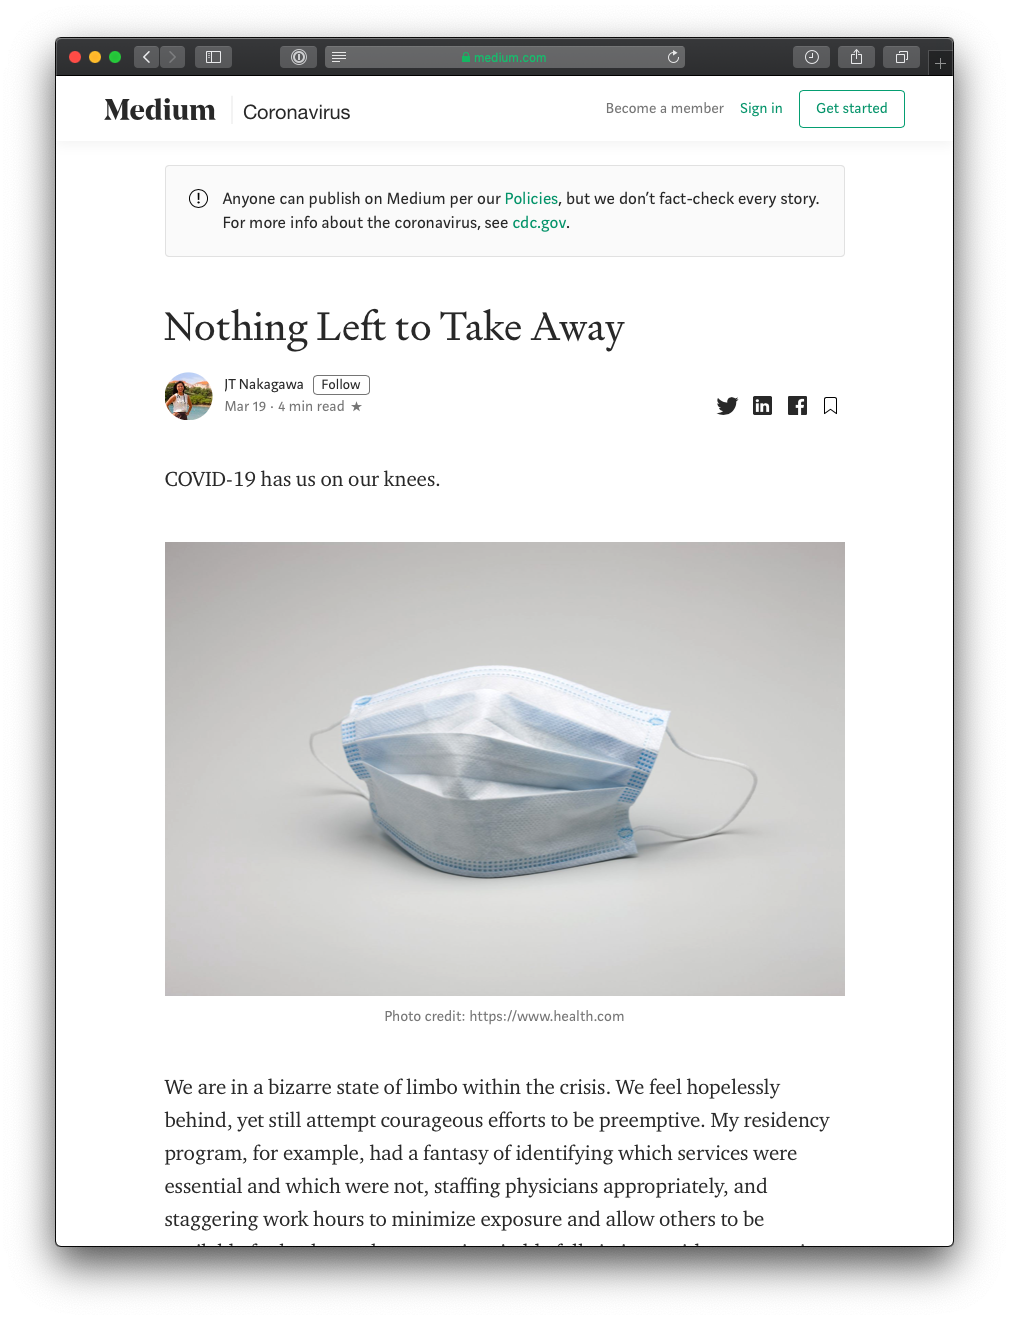
\includegraphics[width=.8\columnwidth]{voorbeeld-medium-desktop}
    \caption{Artikel op Medium weergegeven in een desktop-omgeving}
    \label{fig:ux-voorbeeld-medium:desktop}
\end{figure}

\begin{figure}
    \centering
    \subfloat[Donkere gebruikersomgeving]{{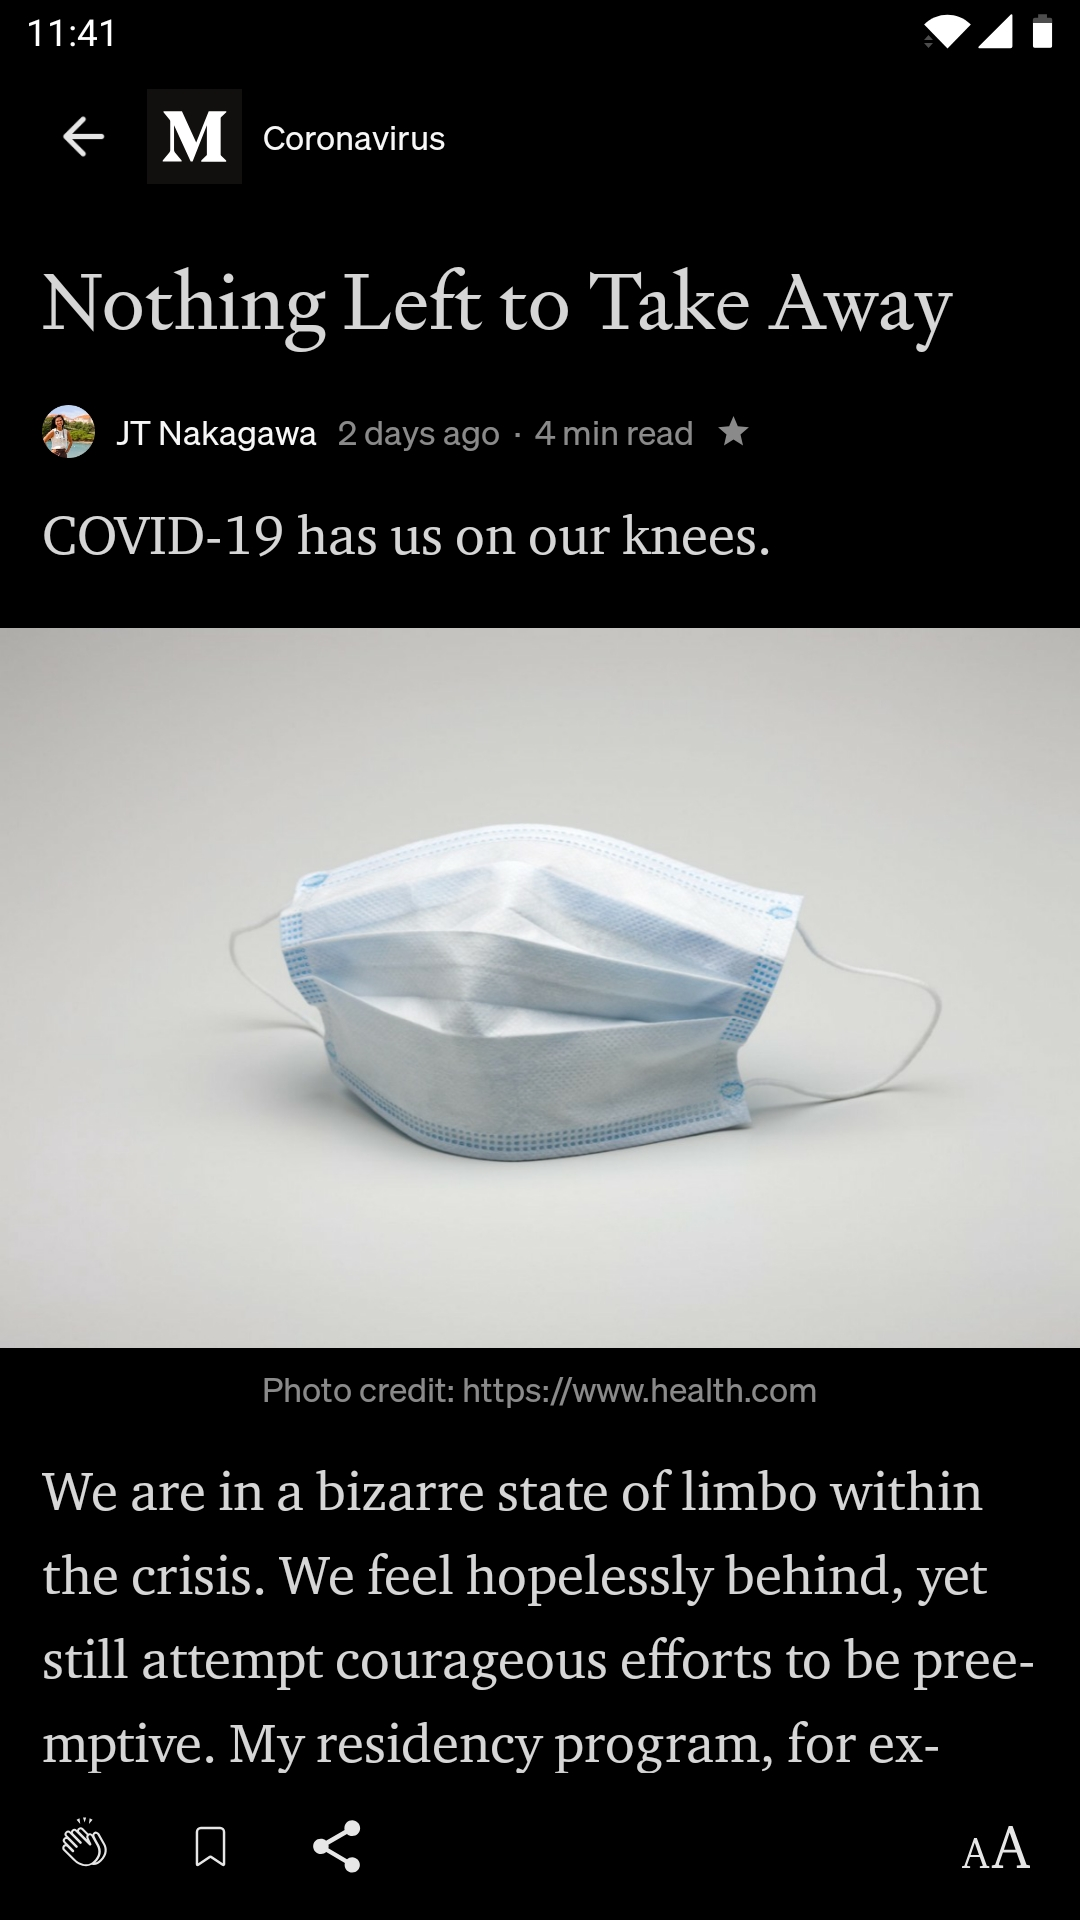
\includegraphics[width=.4\columnwidth]{voorbeeld-medium-mobiel-donker}}}
    \qquad
    \subfloat[Lichte gebruikersomgeving]{{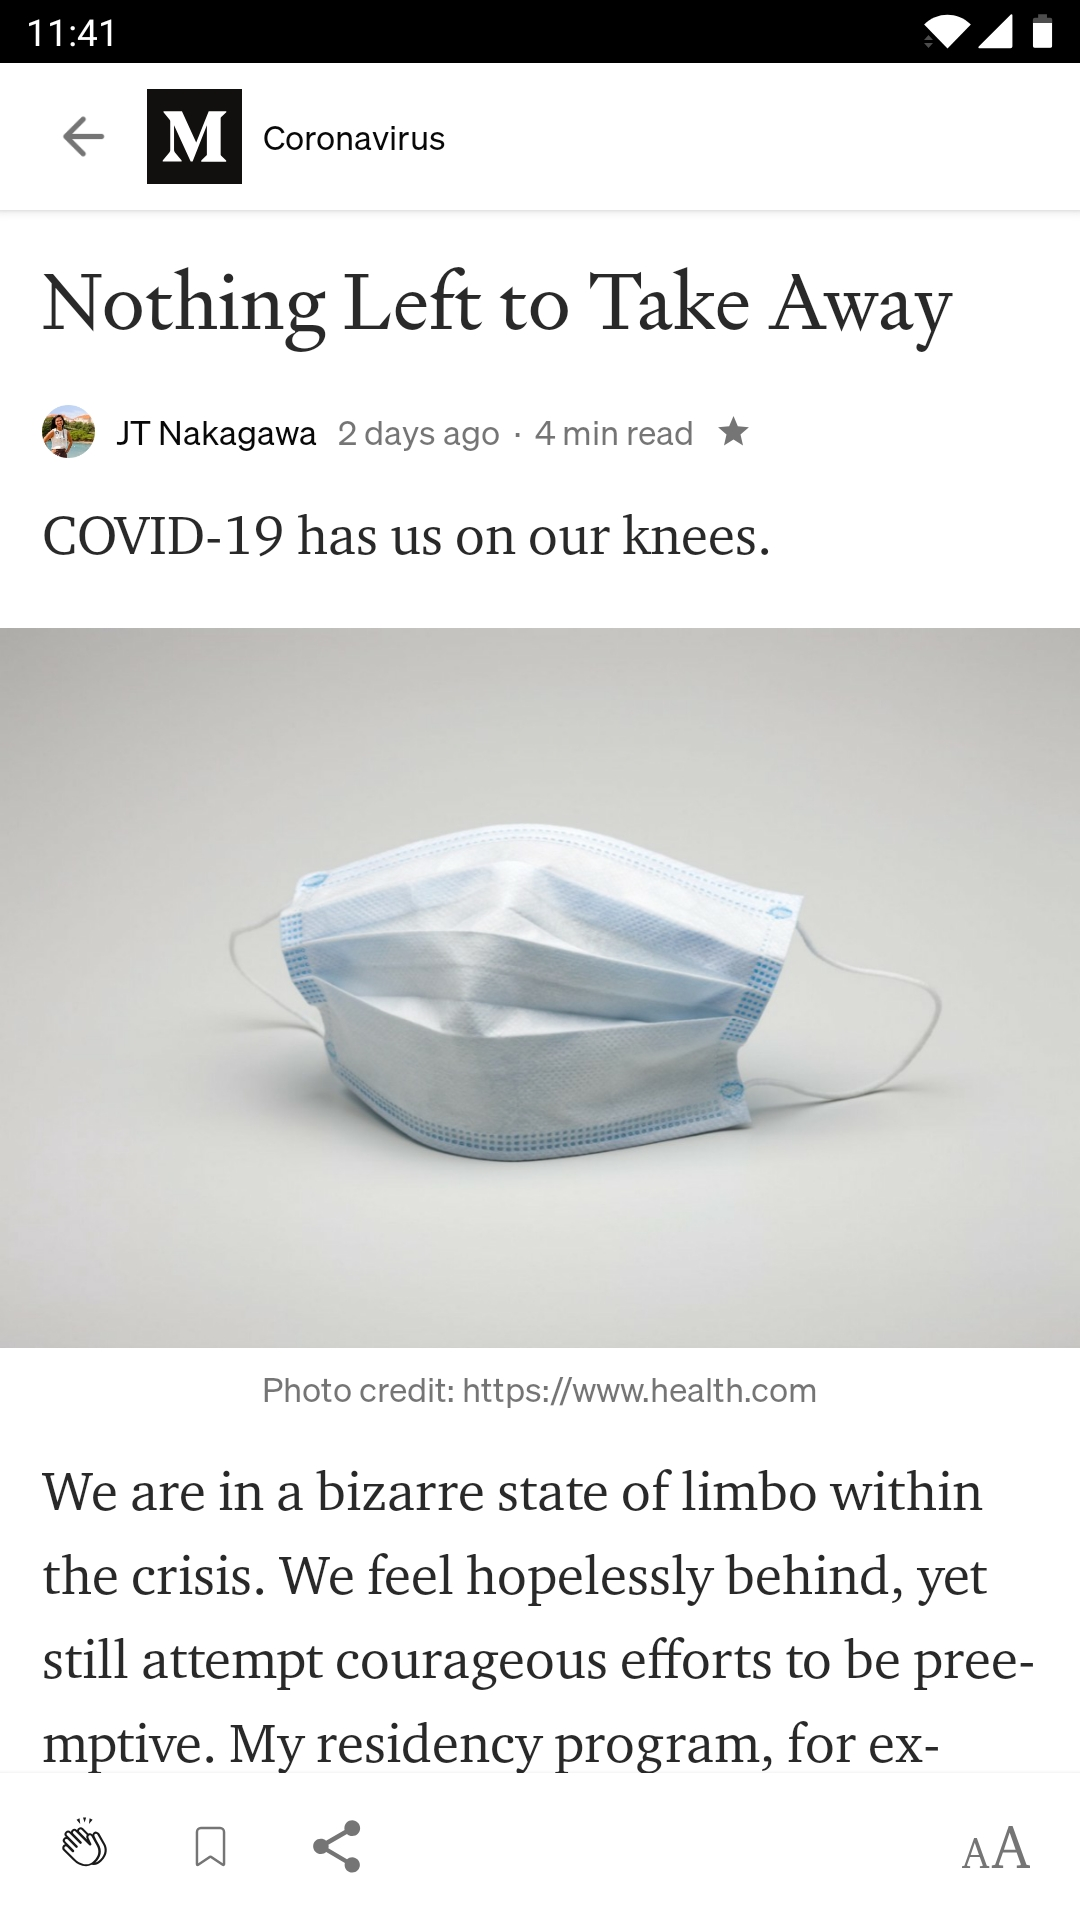
\includegraphics[width=.4\columnwidth]{voorbeeld-medium-mobiel-licht}}}
    \caption{Artikel op Medium weergegeven in een mobiele omgeving}
    \label{fig:ux-voorbeeld-medium:mobiel}
\end{figure}

\textbf{Airbnb} wil verkopen, dat is merkbaar van zodra je de website opent. Airbnb (\url{https://www.airbnb.com/}) is een platform waarmee je een kamer of woning van iemand anders kan huren voor een korte periode. Het is razend populair platform bij mensen die een plezier- of werkreis plannen en iets unieks zoeken of de kosten van hun reis willen drukken. Van zodra je op de homepagina komt zorgt Airbnb ervoor dat je onmiddellijk kan zoeken naar een geschikte plaats om te verblijven op een locatie en tijdstip naar keuze. Gepaard met een uitnodigende titel en een buitengewone afbeelding is de verleiding bij de gebruiker groot om hun ideale trip te beginnen plannen. Door deze directe aanpak vergeet de gebruiker als het ware de concurrentie van Airbnb, wat uiteraard net het doel was van bij het begin.

\begin{figure}
    \centering
    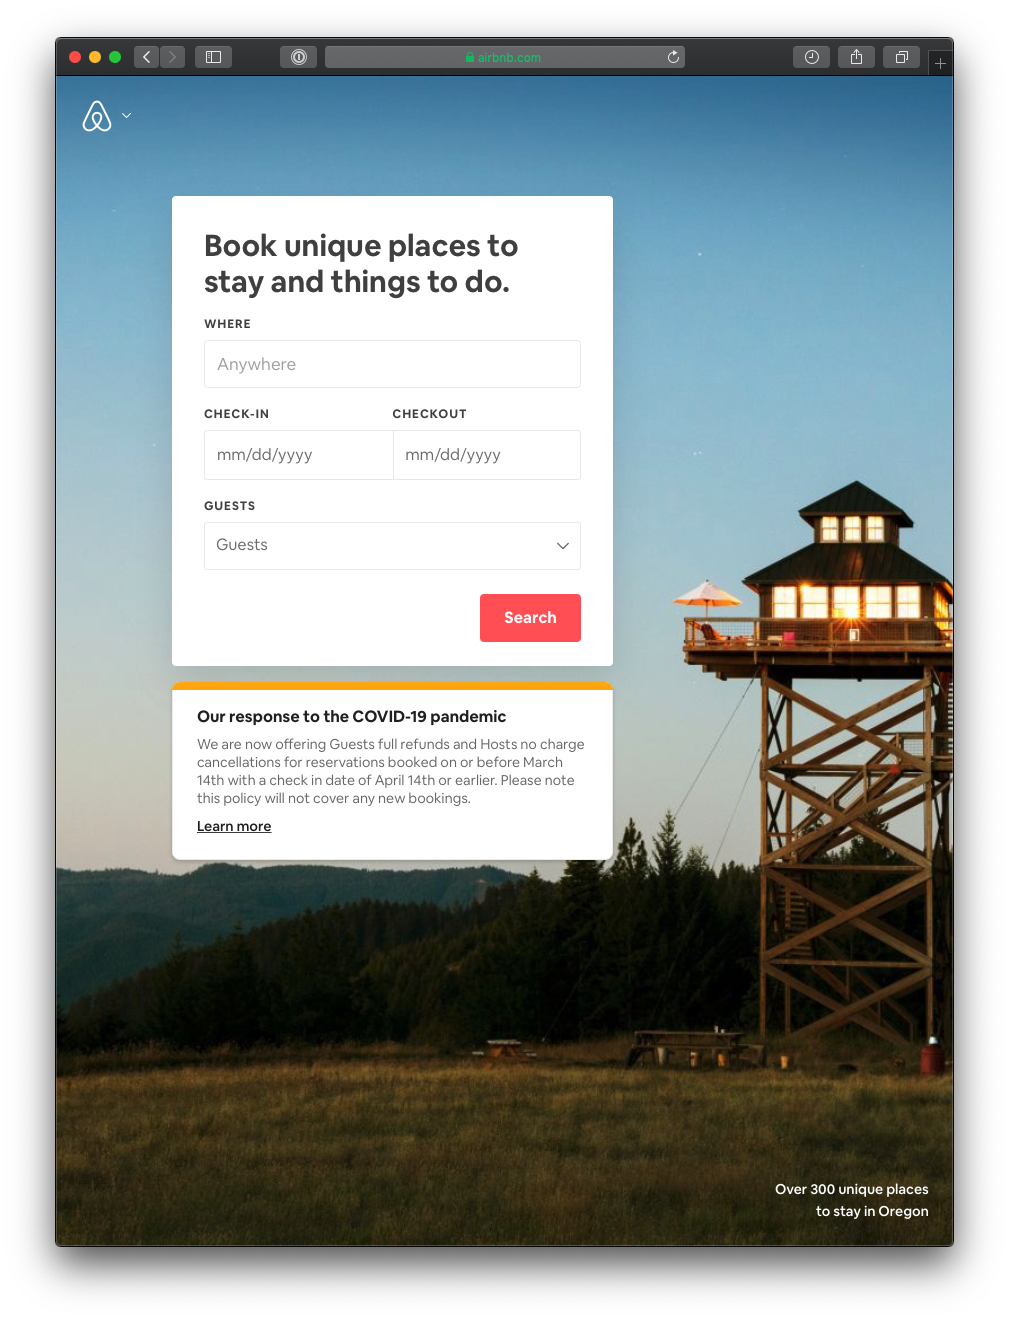
\includegraphics[width=.8\columnwidth]{voorbeeld-airbnb-desktop}
    \caption{Airbnb homepagina}
    \label{fig:ux-voorbeeld-airbnb}
\end{figure}

Slimme apparaten in het huishouden zijn bezig aan een opmars. Eén van de bekendste apparaten is de \textbf{Nest Smart Thermostat}, een slimme thermostaat die verbonden is met het internet. De thermostaat leert wanneer de ruimte moet opwarmen of afkoelen. Het fysieke toestel zelf is de simpliciteit zelve. Het is een grote, ronde knop met centraal de huidige temperatuur, indien de ruimtes opwarmen of afkoelen en de temperatuur waar men naartoe werkt. Een draai naar rechts en je verhoogt de gewenste temperatuur, een draai naar links en je verlaagt deze. De mobiele applicatie bootst deze werking na zodat de gebruiker zich direct comfortabel voelt met de interface (zie figuur~\ref{fig:ux-voorbeeld-nest}).

\begin{figure}
    \centering
    \subfloat[Fysiek toestel]{{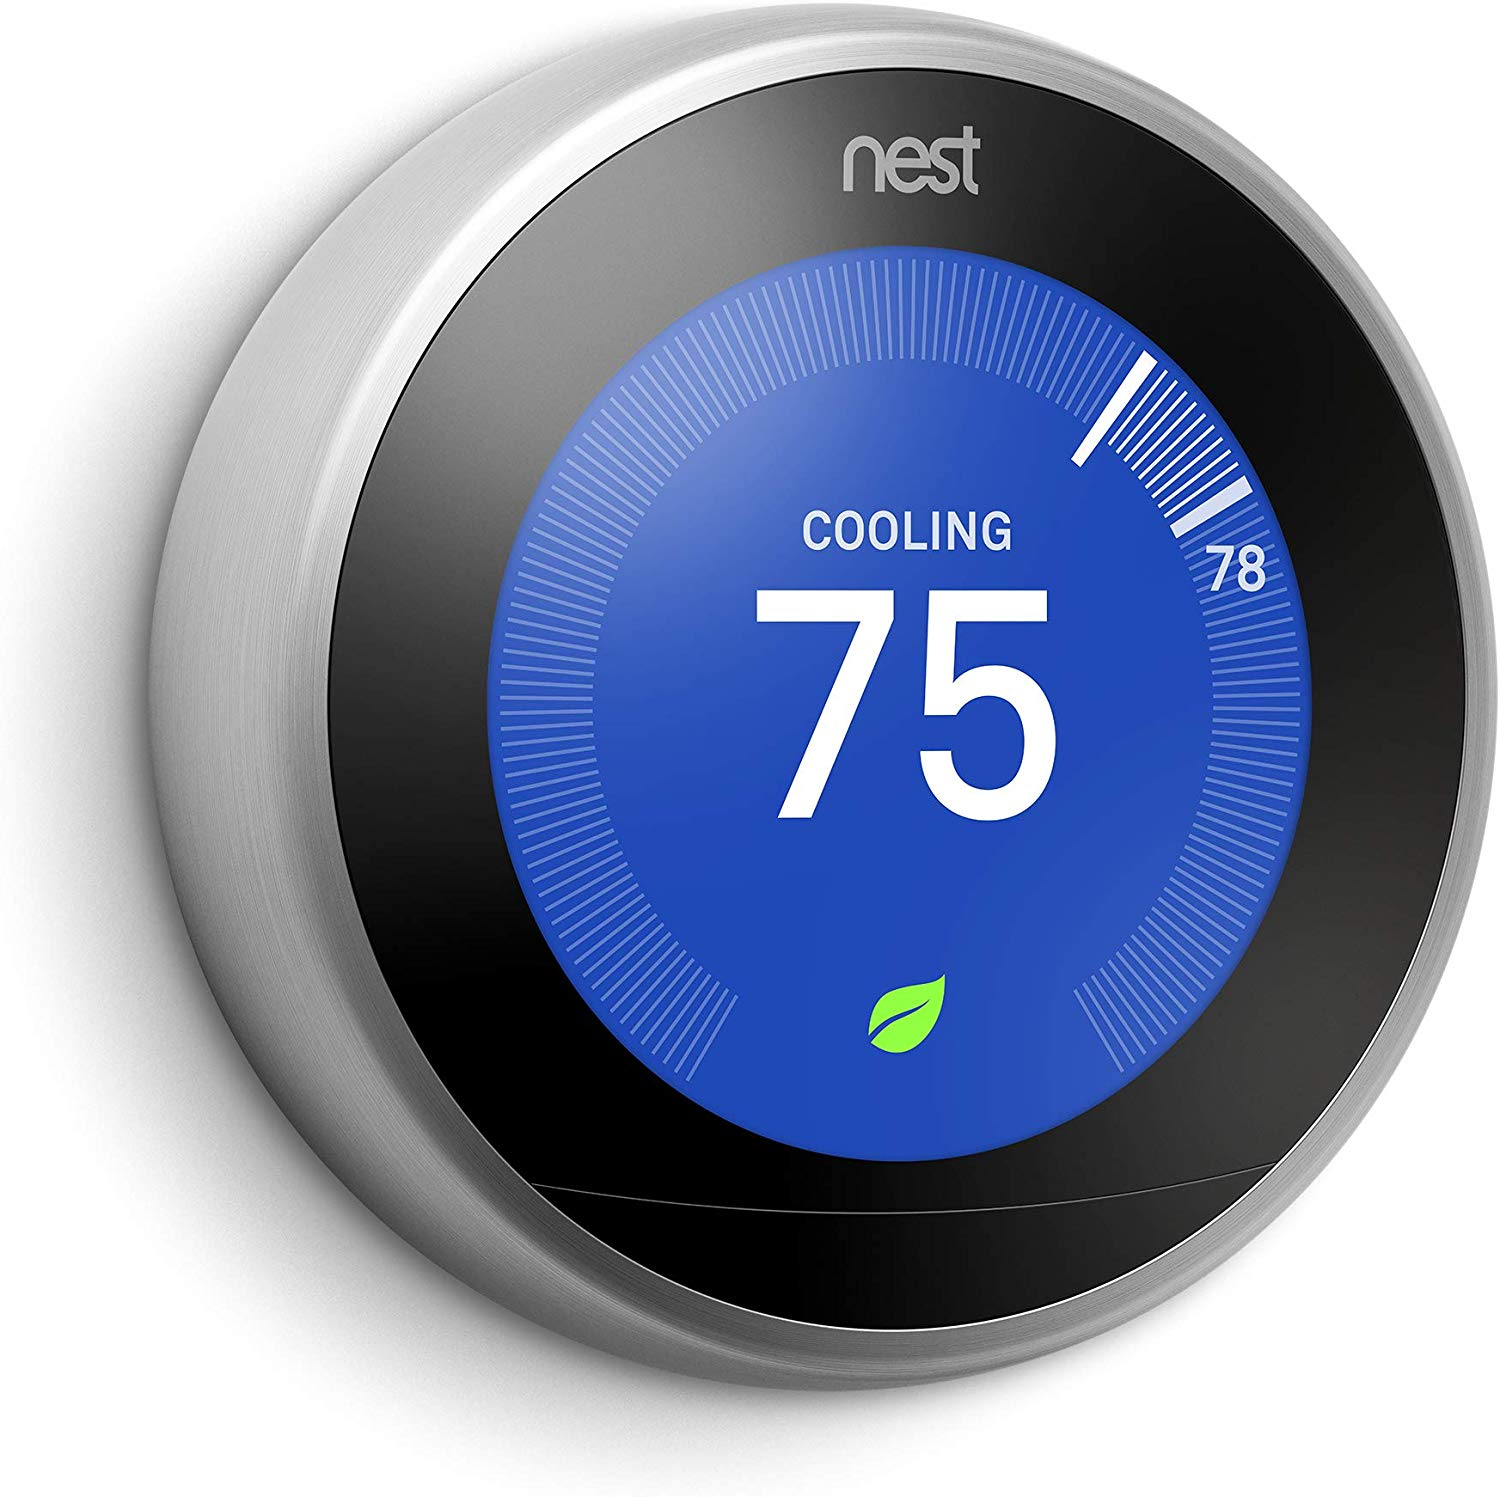
\includegraphics[width=.5\columnwidth]{voorbeeld-nest-toestel}}}
    \qquad
    \subfloat[Mobiele interface]{{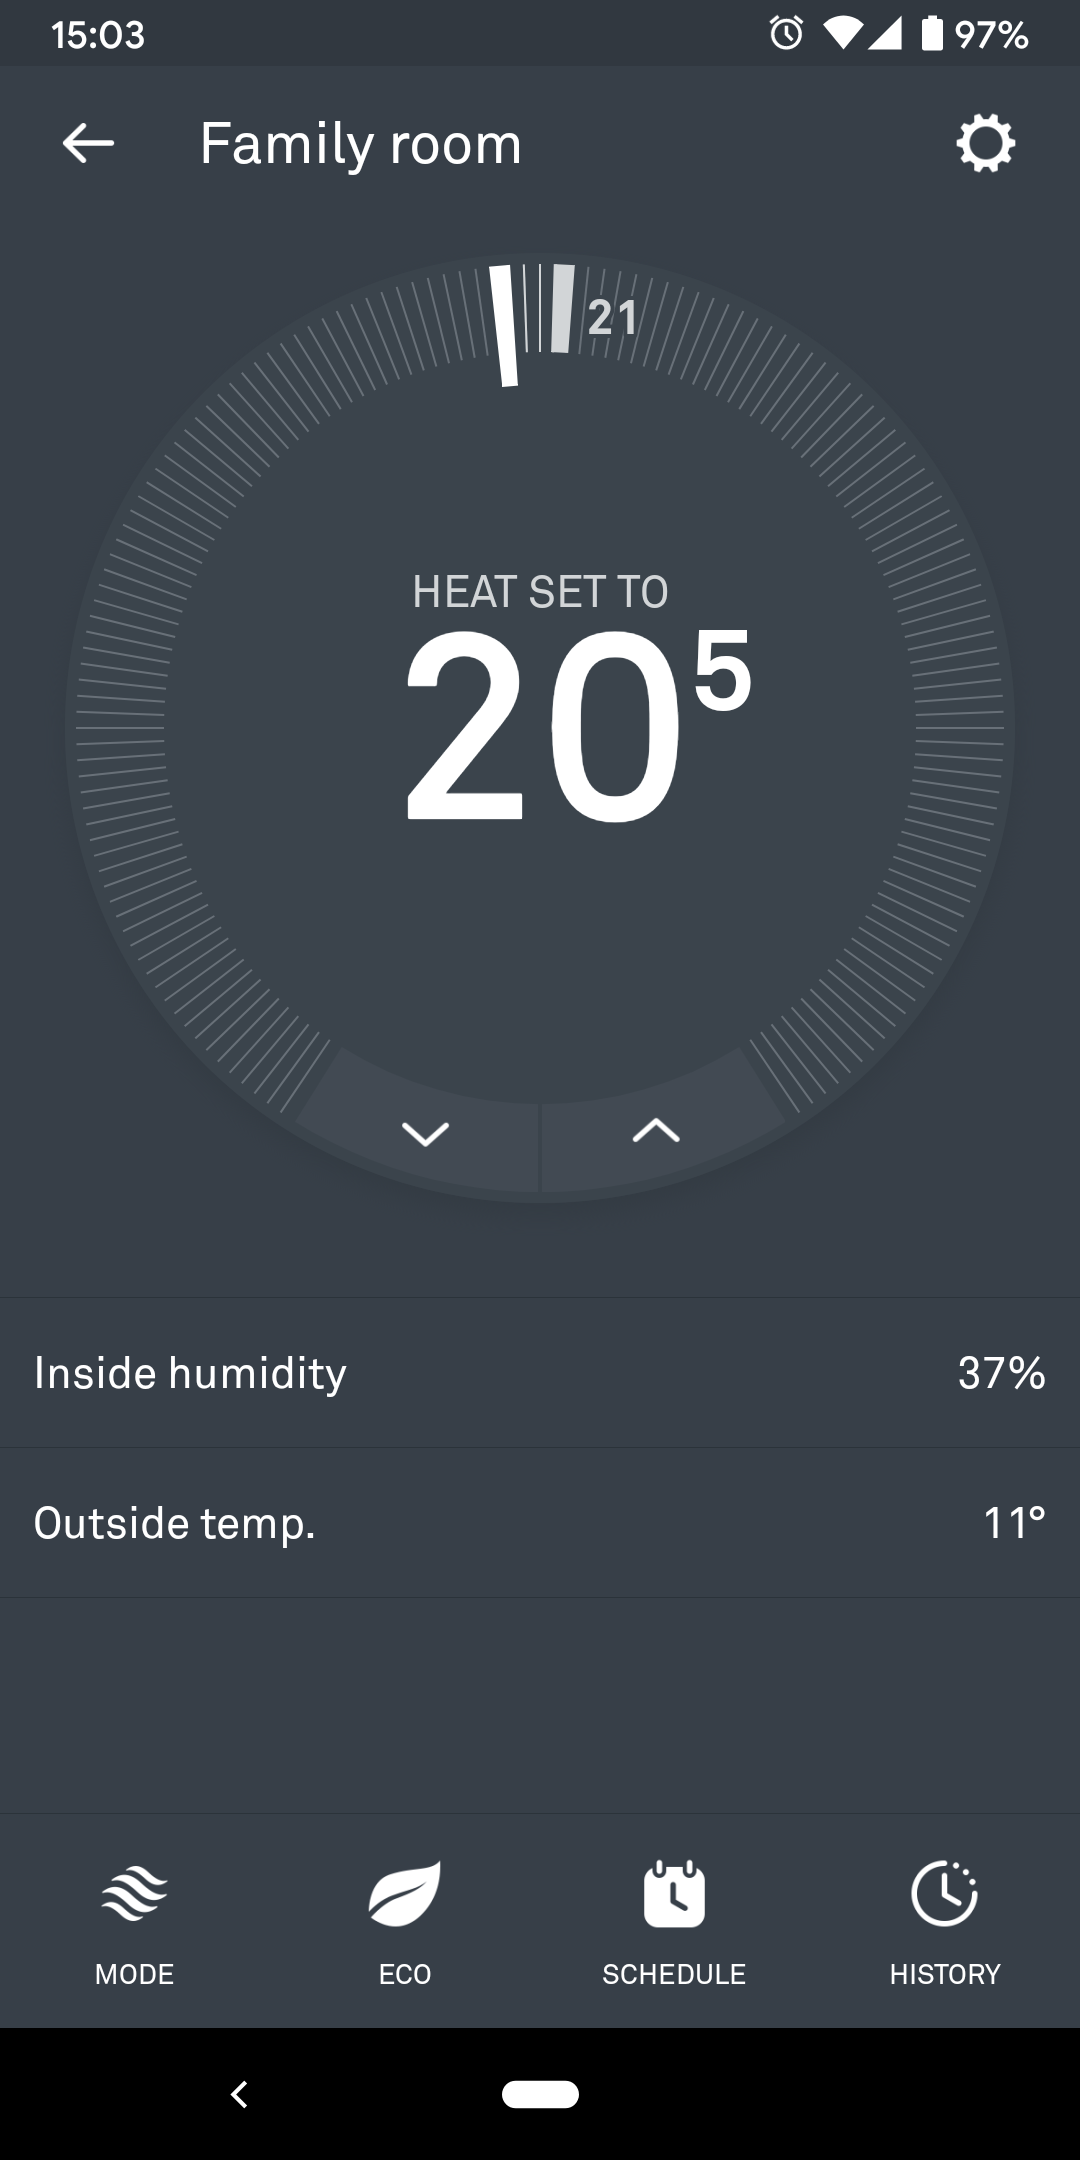
\includegraphics[width=.3\columnwidth]{voorbeeld-nest-mobiel}}}
    \caption{Nest Smart Thermostat}
    \label{fig:ux-voorbeeld-nest}
\end{figure}

\textbf{Hubspot} (\url{https://www.hubspot.com/}) maakt producten voor marketing, sales en klantenservice. Hubspot richt zich tot bedrijven van elke omvang. In dit voorbeeld bekijken we slechts een klein deel van de software. Binnen Hubspot is er de mogelijkheid om een massa-email te plannen die een deel van of alle klanten van de gebruiker bereikt. Uiteraard is dit een actie met een aanzienlijke impact op het bedrijf van de gebruiker. Een verzonden mail kan echter niet ongedaan gemaakt worden. Wanneer de gebruiker de email inplant komt Hubspot met een pop-up melding die toch nog even bevestiging vraagt (zie figuur~\ref{fig:ux-voorbeeld-hubspot}). Deze melding zorgt ervoor dat de kans op fouten verkleind wordt maar ook dat de gebruiker zich gerust voelt bij zijn acties.

\begin{figure}
    \centering
    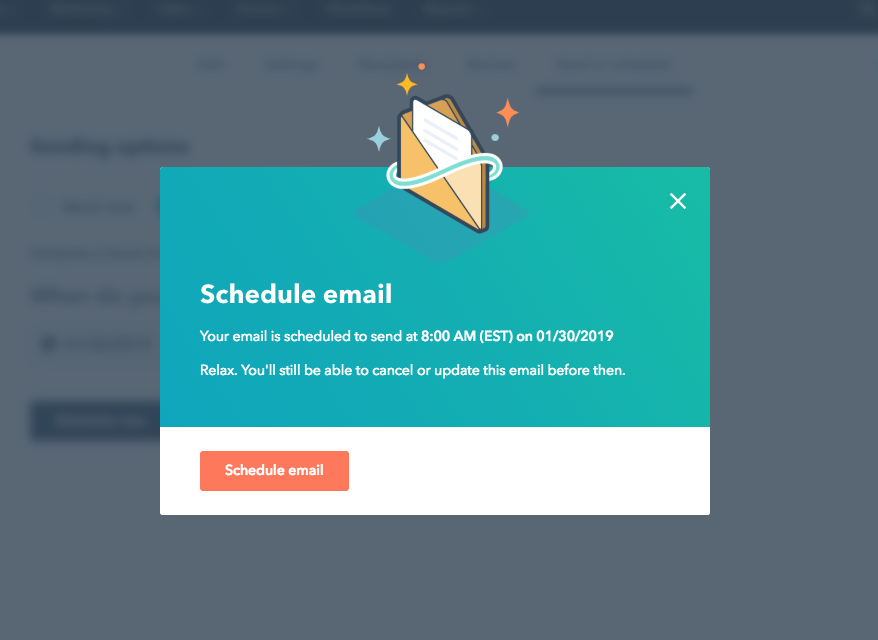
\includegraphics[width=.7\columnwidth]{voorbeeld-hubspot}
    \caption{Hubspot pop-up melding}
    \label{fig:ux-voorbeeld-hubspot}
\end{figure}

\section{Usability testing}
\label{sec:usability-testing}

Usability testing is een methode om alle onderdelen van de user experience honingraat (zie figuur~\ref{fig:ux-facets}) in een applicatie of website te testen. Men test de software in kwestie door er echte gebruikers op te laten werken en ondertussen hun handelingen te observeren. Het doel van usability testing is om de algemene gebruikerservaring te verbeteren~\autocite{Hotjar2020}.

Bij het creëren van software vergeet de ontwikkelaar al snel dat de gewone eindgebruiker vaak meer moeilijkheden zal ondervinden bij het gebruik van zijn creatie dan hijzelf. Doordat de ontwikkelaar hier zelf vaak blind voor is voert men testen uit met de eindgebruiker. Hierdoor kan men een beter inzicht krijgen over hoe bruikbaar de software is. In dit proces worden vaak vele euvels opgemerkt die anders in de productiesoftware zouden aanbelanden.
Zonder usability testing zou men vaak vast komen te zitten met een product dat het team van ontwikkelaars begrijpt, maar de doelgroep niet.

\subsection{Laboratory en field testing}
\label{sec:usability-testing:lab-field-testing}

In voorgaand onderzoek tonen \textcite{Kaikkonen2005} aan dat usability testing onderverdeeld kan worden in twee categorieën, namelijk laboratory en field testing. Laboratory testing houdt in dat men enkele testpersonen uitnodigt in testlabo's, dit is gewoonlijk op kantoor. Dit labo is een rustige ruimte waarin afleidingen beperkt zijn zodat de concentratie gegarandeerd kan worden. Ook al bestaan er veel twijfels rond laboratory testing, volgens \textcite{Kjeldskov2003} wordt het nog steeds vaker verkozen boven field testing. De reden achter deze keuze is vaak omdat men moeilijkheden ondervindt bij field testing. Het is eenvoudiger om testpersonen op te nemen en te observeren bij technieken zoals ``think aloud'' wanneer men gebruik maakt van laboratory testing.

Bij field testing worden te testpersonen uitgenodigd om de applicatie in kwestie te testen in de omgeving waar de applicatie normaal zou gebruikt worden. Een mobiele applicatie zoals \href{https://www.strava.com/}{Strava} die statistieken van lopers en fietsers bijhoudt zou bijvoorbeeld getest worden tijdens een trainingssessie. Sinds de opmars van de smartphone kan field testing steeds meer ingezet worden \autocite{Kjeldskov2004}. De camera die gebruikt wordt om de testsessie op te nemen wordt steeds kleiner, waardoor het field testing een pak aangenamer wordt.

In beide gevallen van usability testing werd geopteerd voor het ``think aloud'' protocol gebaseerd op het werk van \textcite{Ericsson1984}. Hierbij zal de testpersoon luidop denken. Dit zorgt ervoor dat er veel informatie vrijkomt over de gedachtegang van de gebruiker bij het gebruik van de applicatie. Dit kan makkelijk opgenomen worden om later conclusies uit te trekken.

\textcite{Kaikkonen2005} hebben ook kunnen afleiden dat zowel laboratory testing als field testing quasi dezelfde resultaten vertonen. In hun use case werden alle usability fouten bij beide testmethodes gevonden. Bij field testing vond men de fout som wel sneller of kwam men deze meerdere keren tegen.

\subsection{Andere testmethoden}
\label{sec:usability-testing:testmethoden}

Laboratory en field testing zijn slecht twee van vele methodes waarmee de bruikbaarheid van een applicatie kan getest worden. In een artikel van \textcite{Babich2019} worden de zeven belangrijkste methodes opgesomd.

% https://xd.adobe.com/ideas/process/user-testing/top-7-usability-testing-methods/

\subsubsection{Guerilla testing}
\label{sec:usability-testing:testmethoden:guerilla}

Guerilla testing is de eenvoudigste testmethode om zo snel mogelijk resultaten te krijgen. Bij guerilla testing gaat de moderator simpelweg op een publieke plaats aan willekeurige personen vragen om even het prototype van de applicatie te gebruiken. De moderator noteert dan de bevindingen. Guerilla testing voert men het best uit in het begin van het ontwikkelproces, zo weet men snel als men in de juiste richting werkt. Vaak krijgt de testpersoon een kleine attentie na het uitvoeren van de test. Zo kan de moderator bijvoorbeeld in een koffiebar plaatsnemen en testpersonen uitnodigen met een gratis koffie.

\subsubsection{Lab usability testing}
\label{sec:usability-testing:testmethoden:lab}

Deze testmethode werd eerder besproken in hoofdstuk~\ref{sec:usability-testing:lab-field-testing}. In contrast met geurilla testing kan men hier een gerichter publiek aantrekken en kan men zo relevantere informatie verkrijgen.

\subsubsection{Unmoderated remote usability testing}
\label{sec:usability-testing:testmethoden:unmoderated-remote}

Dit is een variant van field testing (zie hoofdstuk~\ref{sec:usability-testing:lab-field-testing}) zonder moderator. Hierbij gebruikt de testpersoon de applicatie in zijn omgeving en op zijn toestel. De informatie die men hierdoor verkrijgt is door het gebrek van een moderator natuurlijk beperkter. Het voordeel van deze methode is dat de kost lager is dan andere testmethoden.

\subsubsection{Contextual inquiry}
\label{sec:usability-testing:testmethoden:contextual-inquiry}

Deze methode leunt meer aan bij een observatiemethode dan bij een testmethode voor usability testing. De testpersonen krijgen hierbij een lijst met vragen die ze moeten beantwoorden over het product. Achteraf worden ze vaak gevraagd de applicatie te gebruiken in hun omgeving met een moderator (zoals bij field testing).

\subsubsection{Phone interview}
\label{sec:usability-testing:testmethoden:phone}

Deze methode is een variant van laboratory testing waarbij men de testpersoon telefonisch opdrachten geeft. Dit gesprek kan opgenomen worden om later conclusies uit te trekken. Bij deze testmethode worden de communicatievaardigheden van de moderator op proef gesteld.

\subsubsection{Card sorting}
\label{sec:usability-testing:testmethoden:card-sorting}

Hierbij worden alle functionaliteiten van de applicatie op kaartjes geschreven. De testpersoon plaats deze kaarten dan in categorieën en geeft deze kaartjes een bepaalde prioriteit. Van zodra de testpersoon aan het werk gaat met de kaartjes moet de moderator uitleg vragen waarom de testpersoon bepaalde kaartjes op een bepaalde plaats legt. 

% TODO

\chapter{\IfLanguageName{dutch}{Methodologie}{Methodology}}
\label{ch:methodologie}

% TODO: Hoe ben je te werk gegaan? Verdeel je onderzoek in grote fasen, en licht in elke fase toe welke stappen je gevolgd hebt. Verantwoord waarom je op deze manier te werk gegaan bent. Je moet kunnen aantonen dat je de best mogelijke manier toegepast hebt om een antwoord te vinden op de onderzoeksvraag.

% TODO - X vervangen

In dit hoofdstuk zal besproken worden hoe het experiment in zijn werk gaat, hoe de steekproef werd getrokken alsook welke variabelen er gemeten werden.

\section{Het experiment}
\label{sec:experiment}

Om te bekijken indien een implementatie van bepaalde learnability technieken invloed heeft op de eindgebruiker zullen er usability tests worden uitgevoerd bij testpersonen. Welke deze testpersonen zijn en hoe er participanten werden verzameld is te raadplegen in hoofdstuk~\ref{sec:experiment:populatie-steekproef}.

Bij dit experiment zal er vooral gefocust worden op laboratory testing (zie hoofdstuk~\ref{sec:usability-testing:lab-field-testing}). Dit wil zeggen dat de testpersoon de applicatie zal testen in het bijzijn van een moderator, maar niet strikt noodzakelijk in de omgeving waarin de applicatie in een reëel scenario gebruikt zou worden. De moderator noteert hierbij alle bevindingen van de testpersoon, alsook waar deze eventueel moeilijkheden ondervindt.

Het experiment zal uitgevoerd worden bij twee groepen. De ene groep krijgt een proof-of-concept applicatie waarin alle learnability technieken in verwerkt zijn. De controlegroep krijgt een applicatie zonder deze learnability elementen. Tijdens deze usability tests wordt van de testpersonen verwacht dat deze een reeks taken tot een goed einde proberen te brengen. Gedurende het experiment worden een aantal variabelen gemeten (zie hoofdstuk~\ref{sec:experiment:variabelen}). De procedure die gevolgd wordt in dit onderzoek is te raadplegen in hoofdstuk~\ref{sec:test-afnemen}.

\subsection{De populatie en steekproef}
\label{sec:experiment:populatie-steekproef}

Aan dit experiment kan quasi iedereen deelnemen indien deze een basiskennis hebben van een smartphone. Leeftijd, afkomst, achtergrond, kennis en andere factoren zijn van weinig belang. Er moet echter wel voldoende variatie zijn. Wanneer de groep participanten enkel uit jonge personen met een technische achtergrond bestaat zal het resultaat sterk beïnvloed worden. Het is dus de bedoeling om zowel jong, oud, technisch onderlegd en technisch leek op te nemen in de poule van participanten.

Participanten worden gezocht zowel in de kring van familie en vrienden als daarbuiten. De resultaten van de laboratory tests met deze participanten gingen normaal aangevuld worden met resultaten uit guerilla tests (zie hoofdstuk~\ref{sec:usability-testing:testmethoden:guerilla}). Deze scriptie werd opgesteld tijdens de Covid-19-situatie en het was dus niet mogelijk en/of veilig om guerilla testing uit te voeren.

Omdat uit veiligheidsoverwegingen geopteerd werd om de test op afstand uit te voeren (de moderator is dus niet fysiek aanwezig bij de testpersoon) moet de testpersoon de proof-of-concept applicatie installeren op hun eigen toestel. De applicatie is geschreven voor het mobiele besturingssysteem van Apple (iOS 13 of hoger) en werd geoptimaliseerd voor gebruik op een smartphone (iPhone of iPod touch). Bij het verzamelen van gegevens van potentiële participanten werd er gevraagd indien deze in het bezit zijn van een toestel dat aan deze voorwaarden voldoet.

Een deelnameformulier werd via verschillende kanalen (sociale netwerken, mond-tot-mondreclame, ...) verspreid om zoveel mogelijk potentiële participanten te bereiken. Het deelnameformulier werd opgesteld in \href{https://forms.office.com/}{Microsoft Forms}. Het volledige formulier is bijgevoegd in bijlage~\ref{bijlage:deelnameformulier}.

In totaal werd het formulier x keer ingevuld. Daaruit werden X personen geselecteerd om deel te nemen aan de test. In figuur~X is te zien in welke leeftijdsgroep de participanten zich bevinden, welk geslacht deze hebben en indien ze zichzelf al dan niet zien als technisch onderlegd.


% TODO - X vervangen
In totaal werd het formulier x keer ingevuld. Daaruit werden x personen geselecteerd om deel te nemen aan de test. In figuur~X is te zien in welke leeftijdsgroep de deelnemers zich bevinden, welk geslacht deze hebben en indien ze zichzelf al dan niet zien als technisch onderlegd.


% Voeg hier je eigen hoofdstukken toe die de ``corpus'' van je bachelorproef
% vormen. De structuur en titels hangen af van je eigen onderzoek. Je kan bv.
% elke fase in je onderzoek in een apart hoofdstuk bespreken.

%\input{...}
%\input{...}
%...

%%=============================================================================
%% Conclusie
%%=============================================================================

\chapter{Conclusie}
\label{ch:conclusie}

% TODO: Trek een duidelijke conclusie, in de vorm van een antwoord op de onderzoeksvra(a)g(en). Wat was jouw bijdrage aan het onderzoeksdomein en hoe biedt dit meerwaarde aan het vakgebied/doelgroep? Reflecteer kritisch over het resultaat. In Engelse teksten wordt deze sectie ``Discussion'' genoemd. Had je deze uitkomst verwacht? Zijn er zaken die nog niet duidelijk zijn? Heeft het onderzoek geleid tot nieuwe vragen die uitnodigen tot verder onderzoek?

In dit onderzoek werd een antwoord gegeven op de onderzoeksvraag ``Kan een (betere) onboarding en in-app user training ervoor zorgen dat de eindgebruiker een beter inzicht heeft op de totale functionaliteit van een grote applicatie?''. Hiervoor werd een proof-of-concept applicatie opgesteld met en zonder learnability-elementen. Deze werd getest door twee groepen participanten.

De resultaten van deze proef gaven aan dat de learnability-elementen zeker hun nut hebben. Echter moet men zeer voorzichtig omspringen met waar en wanneer men deze plaatst. Zoals in hoofdstuk~\ref{ch:stand-van-zaken} werd besproken is het belangrijk om zich te beperken tot de essentie. Frequent de applicatie laten testen om zo te bekijken waar er hulp moet voorzien worden is één van de belangrijkste stappen bij het implementeren van learnability in software.

De verspreiding van help-elementen doorheen de applicatie is een volgend belangrijk aspect bij de implementatie van onboarding en help-elementen. Door de gebruiker niet initieel te overspoelen met info maar deze pas geleidelijk aan nieuwe functionaliteiten aan te leren zal de gebruiker de werking van deze functionaliteiten beter onthouden. De gebruiker zal ook minder snel de aandacht verliezen tijdens bijvoorbeeld een rondleiding.

Er werd voor deze applicatie geen significante relatie gevonden tussen (het gebrek aan) in-app user training en de gebruiksduur en/of levensduur van de applicatie. Wanneer een bedrijf hun software test bij gebruikers die ook effectief een meerwaarde hebben aan de functionaliteiten van deze software kan dit resultaat met hoogste waarschijnlijkheid variëren. Dit kan eventueel bewezen worden in een verder onderzoek.

Een interessante ondervinding uit deze scriptie is het feit dat het mogelijk is de gebruiker aan te zetten tot het gebruik van bepaalde functionaliteiten. Door deze functionaliteiten aan te halen in de onboarding is de gebruiker meer geneigd deze daar uit te proberen en verder te gebruiken. Dit kan interessant zijn om bijvoorbeeld accountcreatie in de kijker te zetten.


%%=============================================================================
%% Bijlagen
%%=============================================================================

\appendix
\renewcommand{\chaptername}{Appendix}

%%---------- Onderzoeksvoorstel -----------------------------------------------

\chapter{Onderzoeksvoorstel}

Het onderwerp van deze bachelorproef is gebaseerd op een onderzoeksvoorstel dat vooraf werd beoordeeld door de promotor. Dat voorstel is opgenomen in deze bijlage.

% Verwijzing naar het bestand met de inhoud van het onderzoeksvoorstel
%---------- Inleiding ---------------------------------------------------------

\section{Introductie} % The \section*{} command stops section numbering
\label{sec:introductie}

Technologie neemt overal de overhand. Meer leeftijdsgroepen maken gebruiken van web- en mobiele applicaties. Deze softwarepakketten worden voor alle mogelijke doeleinden gebruikt, denk maar aan een management platform in een bedrijf, of een mobiel spel om tegen je vrienden te quizzen.

Deze applicaties moeten op een bepaalde manier aan de eindgebruiker uitgelegd worden. Er bestaan verscheidene technieken om alle functionaliteiten binnen de software aan de man te brengen. Boeken deze technieken wel het gewenste resultaat? Is de ene techniek beter dan de andere?

In deze bachelorproef onderzoeken we de onboarding en in-app user training aan de hand van volgende onderzoeksvragen en deelvragen:

\begin{itemize}
    \item Kan een (betere) onboarding en in-app user training ervoor zorgen dat de eindgebruiker een beter inzicht heeft op de totale functionaliteit van een grote applicatie?
    \item Hoe een grote hoeveelheid aan functionaliteiten beheersbaar houden voor de eindgebruiker?
    \item Heeft (het gebrek aan) in-app user training effect op de gebruiksduur en/of levensduur van de applicatie?
    \item Hoe de eindgebruiker wegwijs maken in een grote applicatie?
\end{itemize}

%---------- Stand van zaken ---------------------------------------------------

\section{Literatuurstudie}
\label{sec:state-of-the-art}

\subsection{Wat is 'onboarding'?}
Er bestaan al verscheidene technieken die mogelijks geïmplementeerd kunnen worden in een applicatie om het de gebruiker eenvoudiger te maken deze applicatie te gebruiken. Eén van de bekendste technieken om een gebruiker wegwijs te maken binnen een softwarepakket is 'onboarding'. Onboarding vindt plaats wanneer u de software voor de eerste maal opstart. Het geeft de eindgebruiker een duidelijk inzicht van hoe de applicatie werkt, hoe de functionaliteiten in zijn werk gaan en welke voordelen er worden aangeboden~\autocite{Cardoso2017}.

\subsection{Voorgaand onderzoek}
Bestaand onderzoek bestudeert een manier van onboarding en in-app user training door middel van een 'Learning Center'~\autocite{CamachoHerrero2019}. Hierbij maakt men gebruik van een in-app onderwijsfunctie die de eindgebruiker alle mogelijke functionaliteiten van de software kan uitleggen. Dit platform wil de gebruiker meer betrekken en aanmoedigen om alle elementen te voltooien door middel van gamification elementen zoals checklists of voortgangsbalken. Per onderdeel zelf werd grotendeels gebruik gemaakt van video's die alle uitleg voorzien. In deze bachelorproef zal verder onderzocht worden als het voordeliger is om dit platform op te splitsen in kleine stukken per functionaliteit. Pas wanneer de gebruiker in contact komt met bepaalde functionaliteiten zal de hij de in-app training te zien krijgen.

Onboarding is vaak ook meer dan enkel uitleg over de applicatie. Ook elementen zoals de registratie zijn een stap in het proces om met de software overweg te kunnen~\autocite{renz2014}. Ook een welkomstmail is een veelgebruikt middel om de gebruiker vertrouwd te maken met de applicatie.

Onboarding is verschillend voor webapplicaties als mobiele applicaties~\autocite{RamirezAlvarez2018}. In beide gevallen moet grondig onderzocht worden wat de gebruiker wil bereiken en het gedrag van deze gebruikersgroep is. Applicaties gericht op een jeugdig publiek zullen de onboarding anders aanpakken dan softwarepakketten gericht op het vervullen van een taak in een bedrijfsomgeving.

\subsection{UX testing}
Voorgaand onderzoek maakt duidelijk dat er veel voorbereiding nodig is op vlak van user experience (UX) en usability testing. Om te weten wat de eindgebruiker wil bereiken en welke acties die daarvoor zal ondernemen is er genoeg inlevingsvermogen nodig~\autocite{gualtieri2009}.
Ook mag men er nooit vanuit gaan dat de ontwikkelaar het bij het rechte eind heeft. Hij is immers niet de eindgebruiker en bekijkt de probleemstelling op een andere manier.

%---------- Methodologie ------------------------------------------------------
\section{Methodologie}
\label{sec:methodologie}

Het onderzoeken van technieken zoals in-app user training en bepaalde manieren van het implementeren van deze technieken zal vooral gebeuren aan de hand van experimenten in het kader van usability testing.

Hierbij zal gebruik gemaakt worden van enkele varianten van dummy-applicaties (hetzij met of zonder gebruik van bovenstaande technieken). Gebruikers van de dummy-applicatie zullen fysiek de software doorlopen en enkele opdrachten voltooien. Aan de hand van metingen op basis van een aantal criteria zal kunnen worden besloten of er over een succesvolle test mag gesproken worden. Deze criteria zijn onder meer, maar niet beperkt tot; het succespercentage, het aantal fouten per tijdseenheid, de gemiddelde tijd en de subjectieve tevredenheid van de gebruiker.

De bovengenoemde dummy-applicaties zullen mobiele en/of webapplicaties zijn waarin al dan niet de te onderzoeken technieken geïmplementeerd zullen zijn. Om het onderzoek zo breed mogelijk te houden zal er zowel een applicatie zijn die een software uit de industriële wereld nabootst (denk aan het besturen van een machine, het beheren van bestellingen, ...) als een applicatie voor alledaags gebruik (denk aan een boodschappenlijstje, sociaal netwerk, ...).

Het te onderzoeken doelpubliek zal ook zo breed mogelijk gehouden worden aangezien iedereen ooit wel eens in aanraking komt met software. Het doelpubliek zal nadien opgesplitst worden in doelgroepen op basis van leeftijd en technische kennis.

De gebruikers krijgen enkele opdrachten die ze tot een goed einde moeten brengen op de te testen applicatie. Aan de hand van usability testing zal gemeten worden hoe kwaliteitsvol de software was. De belangrijkste criteria bij deze meting zijn het succespercentage, het aantal fouten per tijdseenheid, de gemiddelde tijd en de subjectieve tevredenheid van de gebruiker. Deze opdrachten zullen formatief verlopen. Er zal dus een moderator/observator aanwezig zijn die noteert hoe de gebruiker de opdrachten uitvoert. Na deze opdrachten zal de gebruiker nog een vragenlijst invullen om zo de SUS-score (System Usability Scale) te berekenen.

%---------- Verwachte resultaten ----------------------------------------------
\section{Verwachte resultaten}
\label{sec:verwachte_resultaten}

Ik verwacht dat de eindgebruiker er gemiddeld langer over zal doen om te wennen aan bepaalde functionaliteiten bij een gebrek aan in-app user training of onboarding. Ook verwacht ik dat een onboarding waarbij alle functionaliteiten aan bod komen een negatieve impact geeft in vergelijking met in-app user training per functionaliteit wanneer de gebruiker hiermee in contact komt.

%---------- Verwachte conclusies ----------------------------------------------
\section{Verwachte conclusies}
\label{sec:verwachte_conclusies}

Het nut van een goede onboarding zal bewezen worden. Alsook mag de onboarding enkel betrekking hebben op de meest essentiële functionaliteit.

In-app user training zal ervoor zorgen dat de eindgebruiker het gevoel heeft de functionaliteit onder de knie te hebben. Daardoor zal de gebruiker minder vlug afstand nemen van de applicatie. Ook zal het eenvoudiger zijn voor gebruikers met een beperkte technische achtergrond om gebruik te maken van de applicatie.



%%---------- Andere bijlagen --------------------------------------------------
% TODO: Voeg hier eventuele andere bijlagen toe
%\input{...}

\chapter{System Usability Scale template}
\label{bijlage:sus}

\includegraphics[page=1,width=.5\columnwidth]{../sus-template/sus-template.pdf}
\includegraphics[page=2,width=.5\columnwidth]{../sus-template/sus-template.pdf}

\chapter{Deelnameformulier}
\label{bijlage:deelnameformulier}
\section{Inleiding}

\textbf{Inschrijving applicatie testing}

Hey!

Bedankt voor je interesse in mijn bachelorproef. Voor mijn onderzoek moet ik enkele usability tests van software uitvoeren. In het kort wil dit dus zeggen dat ik een kleine mobiele applicatie loslaat op echte gebruikers! Na het invullen van deze enquête kom je te weten als je in aanmerking komt voor dit onderzoek.

Wat houdt deze test exact in? Je zal enkele opdrachten moeten uitvoeren op een applicatie die ik zelf ontwikkeld heb, ondertussen bekijk ik aandachtig alle stappen dat je daarvoor onderneemt (no stress, alles wat je doe is juist). Achteraf moet je ook een kleine vragenlijst invullen en stel ik mogelijks nog enkele vragen.

Alvast bedankt!

Vanwege de aanhoudende Covid-19-situatie zal de usability test worden gehouden via een videogesprek.

\section{Mobiel toestel}

\subsection*{Type smartphone in bezit}

Gelieve "iPhone" te selecteren als je tijdelijk een iPhone kan lenen van een vriend, huisgenoot, ...

\begin{itemize}
    \item iPhone
    \item Android-toestel (Samsung, Oneplus, ...) \\ \textit{Bij keuze van deze optie wordt er direct doorverwezen naar sectie~\ref{sec:voldoet-niet}.}
    \item Anders \\ \textit{Bij keuze van deze optie wordt er direct doorverwezen naar sectie~\ref{sec:voldoet-niet}.}
\end{itemize}

\subsection*{Huidige iOS versie}

U vindt uw versie onder Instellingen > Algemeen > Info > Softwareversie

\begin{itemize}
    \item iOS 13.x.x
    \item iOS 12.x.x \\ \textit{Bij keuze van deze optie wordt er direct doorverwezen naar sectie~\ref{sec:voldoet-niet}.}
    \item Lager dan iOS 12.x.x \\ \textit{Bij keuze van deze optie wordt er direct doorverwezen naar sectie~\ref{sec:voldoet-niet}.}
\end{itemize}

\section{Over jezelf}

Jouw apparaat komt in aanmerking voor deze test! Gelieve enkele gegevens over jezelf achter te laten zodat ik jou kan contacteren.

Contactgegevens worden niet gedeeld.

\subsection*{Volledige naam}

Dit is een invulveld.

\subsection*{Leeftijdsgroep}

\begin{itemize}
    \item 70+
    \item 60-69
    \item 50-59
    \item 40-49
    \item 30-39
    \item 20-29
    \item 10-19
\end{itemize}

\subsection*{Geslacht}

\begin{itemize}
    \item Vrouw
    \item Man
    \item Non-binair
\end{itemize}

\subsection*{E-mailadres}

Dit is een invulveld.

\subsection*{Telefoonnummer}

Dit is een invulveld.

\subsection*{Ik heb een computer met een webcam en microfoon}

\begin{itemize}
    \item Ja
    \item Nee
\end{itemize}

\subsection*{Ik identificeer mezelf als technisch onderlegd}

Een smartphone heeft voor mij weinig tot geen geheimen

\begin{itemize}
    \item Ja
    \item Nee
\end{itemize}

\section{Oh nee...}
\label{sec:voldoet-niet}

\textit{Deze sectie wordt enkel getoond indien men niet voldoet aan bepaalde voorwaarden.}

Je komt helaas niet in aanmerking voor deze test. De dummy-applicatie werd geschreven voor iOS-apparaten met versie 13 en hoger. Jouw apparaat voldoet niet aan deze voorwaarden.

\section{Afsluiting}

Bedankt voor de interesse. Indien je jouw contactgegevens hebt moeten achterlaten kom jij in aanmerking voor deze test. In dat geval probeer ik zo snel mogelijk contact met je op te nemen. Vergeet ook niet dit formulier om te delen!

Blijf in uw kot en was uw handen. 

Jakob Lierman


%%---------- Referentielijst --------------------------------------------------

\printbibliography[heading=bibintoc]

\end{document}
